% ----------------------- Project Planning -----------------------------------

\section{Project Planning}

\begin{comment}
    State your project plan with up-to-date tasks, dependencies, timelines and milestones. You may paste your plan appropriately from MS Project etc. 
\vspace{.1in}

\noindent
Include cost analysis if applicable. 
\vspace{.1in}

\noindent
Mention the software life cycle model you followed.    
\end{comment}

\subsection{Software Life Cycle Model}
\noindent
In developing the project, I adopted an iterative approach to the Waterfall model, enabling a structured yet flexible framework for managing the various phases of the project. The project plan outlines specific tasks, dependencies, timelines, and milestones to ensure a systematic progression towards the final goal of analyzing social media posts for mental health disorder detection. \\

\noindent
The Iterative Waterfall model was chosen for this project due to its structured approach while allowing for iterative revisions and refinements. Unlike the traditional Waterfall model, which emphasizes a linear progression through distinct phases, the iterative variant permits revisiting earlier stages based on findings and feedback. This flexibility is particularly beneficial in data-driven projects where insights gained during the analysis may necessitate adjustments to earlier stages, such as refining requirements or enhancing data preparation techniques. \\

\noindent
In this project, the iterative nature of the Waterfall model facilitated ongoing improvement and adaptation throughout the development process. For example, initial results from the model evaluation phase may prompt a revisit to data preprocessing to enhance data quality or to explore alternative modeling techniques. This approach ultimately fosters a more robust final product, ensuring that the developed system meets the dynamic needs of mental health disorder detection in social media posts. \\

\noindent
The key feature of the iterative approach is the feedback loop that exists between the phases. For instance, after completing the testing phase, if certain models do not meet performance expectations, the project can loop back to the implementation phase. This allows for modifications to the models, preprocessing techniques, or even revisiting the requirements to ensure alignment with the project's objectives. \\

\noindent
The project is divided into distinct phases:

\begin{itemize}
    \item \textbf{Requirement Gathering and Analysis} :
    \noindent
    This initial phase involved understanding the project's goals, objectives, and stakeholder expectations. It spanned approximately two weeks, culminating in a detailed requirements document that guided the subsequent stages.
    \item \textbf{Data Collection and Preparation} :
    \noindent
    Utilizing a Twitter sentiment dataset from Kaggle and Reddit API, the data collection phase was executed over a week. This included downloading the dataset, examining its structure, and performing data cleaning and prepossessing to ensure its suitability for analysis.
    \item \textbf{Model Development} :
    \noindent
    This phase, lasting about three weeks, included the creation of a Bag of Words model, splitting the dataset into training and test sets, and implementing various machine learning algorithms such as k-Nearest Neighbors (k-NN) and Support Vector Machines (SVM) for sentiment classification.
    \item \textbf{Model Evaluation} :
    \noindent
    Following model development, a week was allocated for rigorous testing and validation of the models, ensuring they met the required accuracy benchmarks. This phase involved using performance metrics such as accuracy, precision, recall, and F1-score to evaluate the models' effectiveness.
    \item \textbf{Final Deployment and Documentation} :
    \noindent
    The last phase, spanning two weeks, focused on deploying the best-performing model and creating comprehensive documentation. This included user manuals and technical documentation to facilitate future maintenance and enhancements.
\end{itemize}

% Insert SDLC Images
\begin{figure}[h!]  
    \centering
    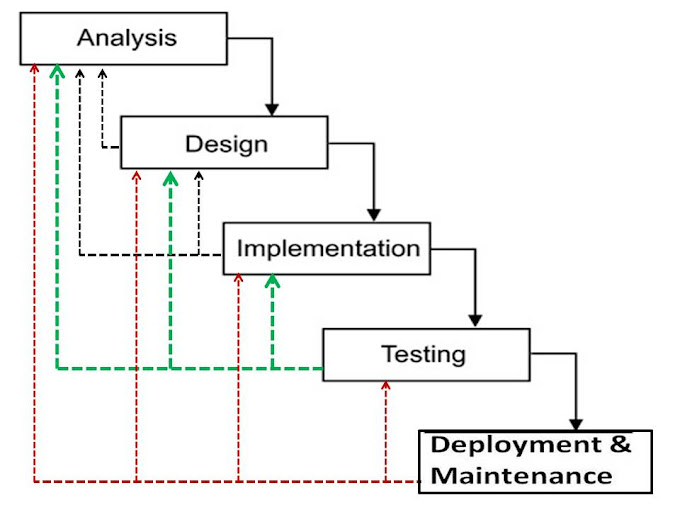
\includegraphics[width=0.6\textwidth]{Images/01 Life_cycle.jpg}  
    \caption{Iterative Waterfall Model}
    \label{Iterative Waterfall Model}  % Label for referencing the figure
\end{figure}


\subsection{Dependencies and Milestones} 
\noindent
Key dependencies were identified for successful project progression. For instance, completion of the data preparation phase was critical before proceeding to model development. Milestones were established at the end of each phase to ensure accountability and track progress. The successful completion of the requirement gathering phase marked the first milestone, followed by the data preparation phase, and so on.

\subsection{Scheduling}
\noindent
Effective scheduling is crucial to the success of any project, as it establishes a clear timeline for tasks, milestones, and dependencies. In the context of our project on detecting mental health disorders through social media analysis, a detailed schedule has been developed to guide the project from inception to completion. This schedule includes specific tasks such as requirement gathering, data preprocessing, model implementation, testing, and deployment, each with clearly defined deadlines. The iterative nature of our chosen methodology allows for flexibility within the schedule, enabling adjustments based on testing outcomes and stakeholder feedback. Key milestones, such as the completion of data analysis, model validation, and user acceptance testing, have been identified to monitor progress and ensure timely delivery of the final product. By utilizing project management tools, such as Microsoft Project, we can visualize and track the progress of tasks, manage resources effectively, and maintain open communication among team members, ensuring that the project stays on schedule and meets its objectives. This proactive approach to scheduling enhances our ability to deliver a high-quality solution that aligns with our goals and stakeholder expectations.

% Insert MS Project Plan Image
\begin{figure}[h!]  
    \centering
    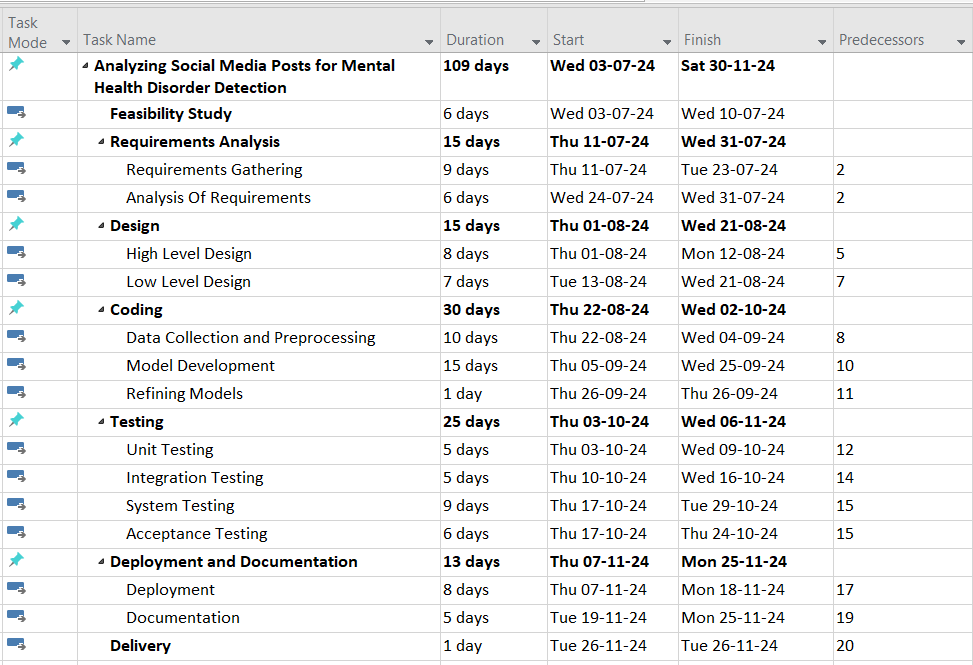
\includegraphics[width=0.9\textwidth]{Images/MS Project Plan Sem 7.png}  
    \caption{Project Plan}
    \label{Project Plan}  % Label for referencing the figure
\end{figure}

\vspace{2cm}

\begin{figure}[h!]  
    \centering
    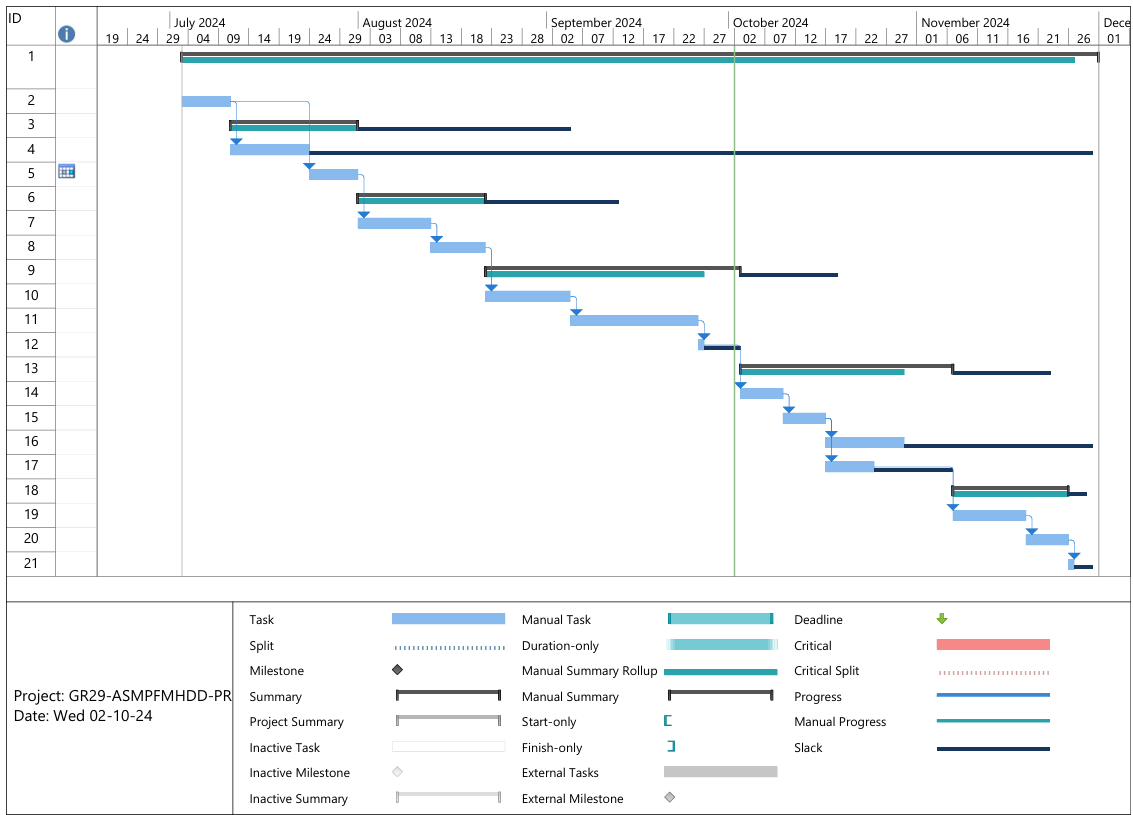
\includegraphics[width=0.9\textwidth]{Images/Gantt Chart.png}  
    \caption{Gantt Chart}
    \label{Gantt Chart}  % Label for referencing the figure
\end{figure}

% ----------------------- Project Planning ends ------------------------------
